\subsection{相对 Stokes 公式（沿纤维积分）}

本号中，X 和 S 表示两个类 \(C^{r}\) 的（实）流形，且 \(\pi: X \to S\) 是一个浸没。我们记 n 为一个整数，并假定对于每个 \(s \in S\)，纤维 \(X_{s} = \pi^{-1}(s)\) 是 \(\pi\) 在 s 处的纤维（它是 X 的子流形（5.10.5）），都是纯 n 维的。

11.4.1. 设 E 和 H 是两个向量空间，F 是 H 的一个 n 维有限维向量子空间。

令 p 为一个满足 \(\geqslant0\) 的整数，令 u 为一个交错的 \((n+p)\)-线性映射，从 \(H^{n+p}\) 到 E，令 \(t_{1},\ldots,t_{p}\) 为 \(H/F\) 的元素；令 \(t_{1}^{\prime},\ldots,t_{p}^{\prime}\) 为 \(t_{1},\ldots,t_{p}\) 在 H 中的代表元。映射

\[
(x _ {1}, \dots , x _ {n}) \mapsto u (t _ {1} ^ {\prime}, \dots , t _ {p} ^ {\prime}, x _ {1}, \dots , x _ {n})
\]

是从 \(\mathbf{F}^n\) 到 E 的 n-线性交错映射，它只依赖于 u 和 \(t_i\)；记作 \(u \perp (t_1, \ldots, t_p)\)（对于特殊情形 \(\mathbf{E} = \mathbf{K}\)，参见 A, III, p. 158）。映射

\[
\left(t _ {1}, \dots , t _ {p}\right) \mapsto u \perp \left(t _ {1}, \dots , t _ {p}\right)
\]

是 p-线性交错的。

11.4.2（“\(\pi\)-扭曲”）。考虑 X 上的向量丛 \(\mathrm{T}(\mathrm{X}/\mathrm{S})\)（8.1.3）；它在 X 的每一点处都有有限秩 n。置 \(\tilde{R}_{\pi} = \tilde{R}_{T(X/S)}\)（10.3.1），\(\tilde{X}_{\pi} = \mathrm{Or}_{T(X/S)}\)（10.2.2）。设 \(s \in S\)；利用 \(\mathrm{T}(\mathrm{X}/\mathrm{S})|_{\mathbf{X}_{s}}\) 与 \(\mathrm{T}(\mathbf{X}_{s})\) 的自然等同（8.1.3），复合映射 \(\tilde{\pi}: \tilde{X}_{\pi} \to S\)（它是 \(\pi\) 与典范映射 \(\tilde{X}_{\pi} \to X\) 的复合）在 s 处的纤维是 \(\tilde{X}_{s}\)（10.2.4）。X 上的 \(\pi\)-扭曲微分形式称为 \(\mathrm{T}(\mathrm{X}/\mathrm{S})\)-扭曲微分形式（10.3.3）。

11.4.3（“S-态射的 S-定向”）。设 \(\mathbf{X}'\) 是一个配备浸没 \(\pi'\colon\mathbf{X}'\to\mathbf{S}\) 的簇，其纤维 \(\mathbf{X}'_{s}\) 都是纯有限维 \(n'\) 维的；设 \(\varphi\colon\mathbf{X}'\to\mathbf{X}\) 是满足 \(\pi'=\pi\circ\varphi\) 的态射。一个 \(\varphi\) 的 S-定向是态射 \(\tilde{\varphi}\colon\tilde{\mathbf{X}}'_{\pi'}\to\tilde{\mathbf{X}}_{\pi}\)，它与群 \(\{\pm1\}\) 的作用交换，并使图表可交换。

\pandocbounded{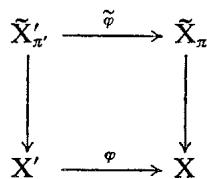
\includegraphics[keepaspectratio]{images/part001_c0391fc0.jpg}}

为 \(\varphi\) 配备 S-定向的数据使得可以像在 10.4.2 中那样，将丛 \(\tilde{\mathbf{R}}_{\pi'}\) 与 \(\varphi^{*}(\tilde{\mathbf{R}}_{\pi})\) 等同，并定义对 \(\pi\)-扭曲微分形式通过 S-定向态射 \(\varphi\) 的拉回；它是 \(\pi'\)-扭曲微分形式，定义在 \(\mathbf{X}'\) 上。

11.4.4. 设 A 是 X 的一个片段，使得 \(\pi\) 在 \(\partial\mathbf{A}\) 上的限制是浸没。对每个 \(s\in\mathbf{S}\)，纤维 \(\mathbf{X}_{s}=\pi^{-1}(s)\) 是与 \(\partial\mathbf{A}\) 横截的 X 的子流形，而 \(\mathbf{A}\cap\mathbf{X}_{s}\) 是 \(\mathbf{X}_{s}\) 的一个片段，记作 \(\mathbf{A}_{s}\)，其边界为 \(\partial\mathbf{A}\cap\mathbf{X}_{s}\)。

令 \(i\) 为将 \(\partial\mathbf{A}\) 典范嵌入 X 的映射。存在唯一一个 S-定向 \(\tilde{i}\)，它是 \(i\) 的定向，使得对于每个 \(s\in\mathbf{S}\)，\(\tilde{i}\) 在 \((\partial\mathbf{A}_{s})^{\sim}\) 上的限制（将其与浸没 \(\partial\widetilde{\mathbf{A}}_{\pi|\partial\mathbf{A}}\to\mathbf{S}\) 在 s 处的纤维等同）是 11.2.1 中定义的、将 \(\partial\mathbf{A}_{s}\) 典范嵌入 \(\mathbf{X}_{s}\) 的映射的定向。若 \(\omega\) 是 X 上的 \(\pi\)-扭曲微分形式，则 \(\omega\) 通过上述带定向的态射 \(i\) 得到的逆像记作 \(\omega|\partial\mathbf{A}\)（参见 11.2.2）。

11.4.5（“内插积”）。令 p 为满足 \(\geqslant 0\) 的整数，令 \(\omega\) 为 X 上取值于以 X 为底空间的向量丛 E 的 \(\pi\)-扭曲微分形式，次数为 \(n + p\)。设 \(s \in S\)，\(x \in X_s\)；有 \(\omega(x) = \xi \otimes u\)，其中 \(\xi\) 是 \(T_x(X_s) = T(X/S)_x\) 的定向，与 \((\tilde{\mathbf{R}}_{X_s})_x = (\tilde{\mathbf{R}}_n)_x\) 中的元素等同（10.3.2），而 u 是一个交错 \((n + p)\)-线性映射，从 \(T_x(X)\) 到 \(E_x\)。令 \(t_1, \ldots, t_p\) 为 s 处 S 的切向量。置

\[
\theta (x) = \xi \otimes (u \llcorner (t _ {1}, \dots , t _ {p})) \in (\tilde {\mathbf {R}} _ {\mathrm{X} _ {s}}) _ {x} \otimes (\mathrm{Alt} ^ {n} (\mathrm{T} (\mathrm{X}); \mathrm{E})) _ {x}
\]

（参见 11.4.1）。于是得到 \(\theta: x \mapsto \theta(x)\)，它是 \(X_s\) 上的一个次数为 n 的扭曲微分形式，取值于 \(E|_{X_{s}}\)。将其记作 \(\omega \perp (t_1, \ldots, t_p)\)。

特别地，设 M 是以 S 为底空间、类 \(C^{r-1}\) 的向量丛，并取 \(E = \pi^{*}(M)\)。丛 \(E|_{X_{s}}\) 自然地可与以 \(X_{s}\) 为底、由 Banach 空间 \(M_{s}\) 定义的平凡丛等同，而形式 \(\omega\perp(t_{1},\ldots,t_{p})\) 可与 \(X_{s}\) 上取值于 \(M_{s}\) 的扭曲微分形式等同。

11.4.6. 保留前述记号（特别是 \(E=\pi^{*}(M)\)），并进一步假定 X 是分离的且 \(\omega\) 是连续的。设 A 是 X 的一个片段，使得 \(\pi\) 在 \(\partial A\) 上的限制是浸没，且 \(\pi\) 在 A 与 \(\omega\) 的支集的交上的限制是本原的。对于 \(s \in S\) 和 \(t_{1},\ldots,t_{p}\in\mathrm{T}_{s}(\mathrm{S})\)，形式 \(\omega \perp (t_{1}, \ldots, t_{p})\)（11.4.5）是 \(X_{s}\) 上连续的 n 次扭曲微分形式，取值于 Banach 空间 \(M_{s}\)，并且其支集与 \(A_{s}\) 的交是紧的。存在唯一一个 S 上取值于向量丛 M 的 p 次微分形式 \(\alpha\)，使得

\[
\alpha (s) \left(t _ {1}, \dots , t _ {p}\right) = \int_ {\mathrm{A} _ {s}} \omega \perp \left(t _ {1}, \dots , t _ {p}\right)
\]

对于所有 \(s \in S\) 和 \(t_{1},\ldots,t_{p}\in\mathrm{T}_{s}(\mathrm{S})\) 都成立。形式 \(\alpha\) 记作 \(\int_{\pi|\mathbf{A}} \omega\)（或简记为 \(\int_{\pi} \omega\)，当 \(\mathbf{A} = \mathbf{X}\) 时）；称它为对 \(\omega\) 在 \(\mathbf{A}\) 上沿 \(\pi\) 的纤维积分所得的形式。若 \(\omega\) 属于类 \(\mathbf{C}^{k}\)（\(0\leqslant k\leqslant r-1,\ k\leqslant\omega\)），则 \(\int_{\pi|\mathbf{A}} \omega\) 也属于同一类。

当 \(\omega\) 是次数 \(< n\) 的形式时，约定 \(\int_{\pi|\mathbf{A}} \omega = 0\)。

11.4.7. 保留前述假设和记号。

\begin{enumerate}
\def\labelenumi{\alph{enumi})}
\tightlist
\item
  对于 S 上的每个连续标量微分形式 \(\beta\)，有
\end{enumerate}

\[
\int_ {\pi | \mathrm{A}} (\pi^ {*} \beta) \wedge \omega = \beta \wedge \int_ {\pi | \mathrm{A}} \omega .
\]

\begin{enumerate}
\def\labelenumi{\alph{enumi})}
\setcounter{enumi}{1}
\tightlist
\item
  令 \(\eta\) 是 X 上的连续向量场，\(\zeta\) 是 S 上的连续向量场，并且 \(\eta\) 关于 \(\pi\) 与 \(\zeta\) 相关（8.2.6）。有
\end{enumerate}

\[
i (\zeta) \int_ {\pi | \mathrm{A}} \omega = \int_ {\pi | \mathrm{A}} i (\eta) \omega .
\]

\begin{enumerate}
\def\labelenumi{\alph{enumi})}
\setcounter{enumi}{2}
\tightlist
\item
  进一步假设 \(\eta\)、\(\zeta\) 和 \(\omega\) 属于类 \(\mathbf{C}^1\)，且有 \(\eta(x) \in \mathrm{T}_x(\partial \mathbf{A})\) 对所有 \(x \in \partial \mathbf{A}\) 成立，并且 \(\mathbf{M}\) 是由 Banach 空间 E 定义的平凡丛。我们有
\end{enumerate}

\[
\theta_ {\zeta}. \int_ {\pi | \mathrm{A}} \omega = \int_ {\pi | \mathrm{A}} \theta_ {\eta}. \omega ,
\]

（参见 8.4.2 和 10.3.4）。

\begin{enumerate}
\def\labelenumi{\alph{enumi})}
\setcounter{enumi}{3}
\tightlist
\item
  若 \(\omega\) 的次数为 \(n + p\) 且属于类 \(\mathbf{C}^1\)，则有
\end{enumerate}

\[
d \left(\int_ {\pi | \mathrm{A}} \omega\right) = \int_ {\pi | \mathrm{A}} d \omega + (- 1) ^ {p} \int_ {\pi | \partial \mathrm{A}} \omega | \partial \mathrm{A}.
\]

\begin{enumerate}
\def\labelenumi{\alph{enumi})}
\setcounter{enumi}{4}
\tightlist
\item
  假设 S 退化为一点。此时 X 上的 \(\pi\)-扭曲形式就是通常的扭曲形式（10.4.1）。若 \(\omega\) 的次数为 \(n\)，则 S 上的 0 次形式 \(\int_{\pi|A} \omega\) 是常数 \(\int_{A} \omega\)（10.4.3）。
\end{enumerate}

11.4.8. 设 \(\pi': S \to S'\) 是一个浸没；其 \(\pi'\) 的纤维是维数恒定且有限的纯 \(n'\) 维子流形。置 \(\pi'' = \pi' \circ \pi\)；它是 X 到 \(S'\) 的一个浸没，其纤维是维数 \(m = n + n'\) 的纯子流形。

设 \(x\in X\)。序列

\[
0 \longrightarrow \mathrm{T} (\mathrm{X} / \mathrm{S}) _ {x} \stackrel {\mathrm{Id}} {\longrightarrow} \mathrm{T} (\mathrm{X} / \mathrm{S} ^ {\prime}) _ {x} \stackrel {\mathrm{T} _ {x} (\pi)} {\longrightarrow} \mathrm{T} (\mathrm{S} / \mathrm{S} ^ {\prime}) _ {\pi (x)} \longrightarrow 0
\]

是正合的。存在唯一一个同构 \(j\)，它从向量丛 \(\tilde{\mathbf{R}}_{\pi} \otimes \pi^{*}(\tilde{\mathbf{R}}_{\pi'})\) 到 \(\tilde{\mathbf{R}}_{\pi'}\)，使得若 \(\xi\)（相应地 \(\eta\)）是 \(\mathrm{T}(\mathrm{X}/\mathrm{S})_x\)（相应地 \((\pi^{*}\mathrm{T}(\mathrm{S}/\mathrm{S}'))_x\)，将其与 \(\mathrm{T}(\mathrm{S}/\mathrm{S}')_{\pi(x)})\) 等同）的一个定向，则 \(j(\xi \otimes \eta) = \eta\xi\)（乘积由前述正合序列（10.2.1）定义）。

令 M' 是以 S' 为底空间的向量丛；置 \(\mathbf{M} = \pi'^{*}(\mathbf{M}')\)，且 \(\mathbf{E}=\pi^{*}(\mathbf{M})=\pi''^{*}(\mathbf{M}')\)。若 \(\omega\) 是 X 上取值于 E 的 \(\pi''\)-扭曲微分形式，则利用同构 j，可将其与一个 \(\pi\)-扭曲形式等同，该形式取值于 \(\pi^{*}(\tilde{\mathbf{R}}_{\pi'}) \otimes \mathbf{E}\)，或等价地，与取值于 \(\pi^{*}(\tilde{\mathbf{R}}_{\pi'} \otimes \mathbf{M})\) 的形式等同。

再设 A 是 X 的一个片段，使得 \(\pi|\partial\mathrm{A}:\partial\mathrm{A}\to\mathrm{S}\) 是浸没；于是 \(\pi''|\partial\mathrm{A}:\partial\mathrm{A}\to\mathrm{S}'\) 也如此。进一步假设 \(\omega\) 连续，且 \(\pi''\) 在 \(\mathbf{A}\cap\operatorname{Supp}\omega\) 上的限制是本原的；则 \(\pi\) 在 \(\mathbf{A}\cap\operatorname{Supp}\omega\) 上的限制也如此。一方面，可以考虑微分形式 \(\int_{\pi''|\mathrm{A}}\omega\) 在 \(\mathrm{S}'\) 上，它取值于 \(\mathrm{M}'\)；另一方面，可以考虑微分形式 \(\int_{\pi|\mathrm{A}}\omega\) 在 \(\mathrm{S}\) 上，它是取值于 \(\tilde{\mathbf{R}}_{\pi'}\otimes\mathrm{M}\) 的形式，或等价地，是一个 \(\pi'\)-扭曲形式，取值于 \(\mathbf{M}=\pi'^{*}(\mathbf{M}')\)。此外，\(\pi(\mathrm{A})\) 是 \(\mathrm{S}\) 的一个开子流形，且 \(\pi'\) 在 \(\pi(\mathrm{A})\cap\mathrm{Supp}\int_{\pi|\mathrm{A}}\omega\) 上的限制是本原的。形式 \(\int_{\pi'|\pi(\mathrm{A})}\int_{\pi|\mathrm{A}}\omega\) 有定义；它是 \(\mathrm{S}'\) 上取值于 \(\mathrm{M}'\) 的微分形式。有

\[
\int_ {\pi^ {\prime} \circ \pi | A} \omega = \int_ {\pi^ {\prime} | \pi (A)} \int_ {\pi | A} \omega .
\]

若 A = X，则有

\[
\int_ {\pi^ {\prime} \circ \pi} \omega = \int_ {\pi^ {\prime}} \int_ {\pi} \omega .
\]

